% Gemini theme
% https://github.com/anishathalye/gemini

\documentclass[final]{beamer}

\usepackage[size=custom,width=84,height=119,scale=0.65]{beamerposter}

\usetheme{gemini}
\usecolortheme{gemini}
\usepackage{graphicx}
\usepackage{anyfontsize}

\usefonttheme{serif}

\usepackage{tgadventor}
\renewcommand*\familydefault{\sfdefault} %% Only if the base font of the document is to be sans serif
\usepackage[T1]{fontenc}

\usepackage{setspace}
\doublespacing

% Upscaling the math formulas. Matches on a original size thus it needs to be found out
% which can be done with:
% \normalsize
%The value of \textbackslash normalsize is \makeatletter\f@size pt\makeatother.
\DeclareMathSizes{16.17}{22}{16}{14}  % Increase math sizes

% ====================

% If you have N columns, choose \sepwidth and \colwidth such that
% (N+1)*\sepwidth + N*\colwidth = \paperwidth
\newlength{\sepwidth}
\newlength{\colwidth}
\setlength{\sepwidth}{0.025\paperwidth}
\setlength{\colwidth}{0.3\paperwidth}

\newcommand{\separatorcolumn}{\begin{column}{\sepwidth}\end{column}}

% ====================
% Title
% ====================

\title{PeaceFounder: EVoting by\\ Pseudonym Braiding}

\author{Dr. Janis Erdmanis}

\institute[shortinst]{janiserdmanis@protonmail.ch}

% ====================
% Footer (optional)
% ====================

\footercontent{
  \href{https://www.janiserdmanis.org}{janiserdmanis.org} \hfill
  EVoteID 2023, Luxemburg \hfill
  \href{mailto:janiserdmanis@protonmail.ch}{janiserdmanis@protonmail.ch}}
% (can be left out to remove footer)

% ====================
% Logo (optional)
% ====================

% use this to include logos on the left and/or right side of the header:
% \logoright{\includegraphics[height=7cm]{logo1.pdf}}
% \logoleft{\includegraphics[height=7cm]{logo2.pdf}}

% ====================
% Body
% ====================

%\setlength{\intextsep}{0pt plus 2pt minus 2pt} 

\begin{document}

% \normalsize
% The value of \textbackslash normalsize is \makeatletter\f@size pt\makeatother.

\begin{frame}[t]
\begin{columns}[t]
\separatorcolumn

\begin{column}{\colwidth}

\vspace{-5cm}
  
\begin{block}{Braid Proof}

Braiding is a cryptographic scheme that shuffles input pseudonyms $y_i = g^{x_i}$ and exponentiates them with a secret factor $s$, resulting in output pseudonyms $y^\prime_i=(g^{x_i})^s = (g^s)^{x_i}=h^{x_i}$ on a new relative generator $h = g^s$. Private key owners $x_i$ can use the relative generator $h$ to issue cryptographic signatures with the new pseudonyms without being linked to the input pseudonyms. To ensure integrity, braiding is supported with zero-knowledge proof, represented as a knot in the image below. 

\begin{center}
  \vspace{-0.5cm}
  \includegraphics[width=0.8\colwidth]{figures/braid.pdf}
  \vspace{-1cm}
\end{center}

The braid proof is constructed from zero-knowledge proof of shuffle and proof of decryption. Let's consider a set of members' pseudonyms $\{y_i\}$ as elements from a cryptographic group $y_i \in G$ on a relative generator $g \in G$. The braider computes a set of output pseudonyms with the following steps: 

\begin{enumerate}
\item Generates a secret exponentiation factor $s$ 
\item Computes a new relative generator $h \leftarrow g^s$ 
\item Calculates ElGamal reencryption shuffle on the pseudonym set as $\{(a_i, b_i)\} \leftarrow \mathsf{Shuffle}_g(\{(h, y_i)\})$
\item Decrypts $c_i \leftarrow b_i^s$
\item Computes the resulting pseudonyms as $y_i^\prime = c_i/a_i$
\end{enumerate}

Step 3 is supplemented with a zero-knowledge proof of shuffle, whereas steps 2 and 4 with a proof of decryption. These proofs form a braid proof represented as a knot in the picture.  

This procedure was first introduced in the work of Haeini \& Spycher. Here, a slight variation of it is shown, which streamlines implementation as it avoids the identity element. A Verificatum-compatible proof of shuffle for step 3 and a custom implementation for proof of decryption in steps 2 and 4 are used, both implemented in Julia and available in the {\it ShuffleProofs.jl} package.
  
\end{block}

\begin{block}{History Tree}

  A history tree was proposed by Crosby \& Wallach that enables ledger auditing without the need for complete replication. By committing to the root of this tree, the bulletin board can be held accountable for the integrity and immutability of the records.
  
  \begin{itemize}
  \item {\bf Inclusion Proof:} History trees provide efficient backtracking hash chain proofs of any record's inclusion with respect to the current tree root commit. Clients get inclusion proofs along with records to verify their authenticity.
  \item {\bf Consistency Proof:} This proof safeguards ledger immutability over time. It proves that a current bulletin board commit retains all records from its previous commit, with new records appended. This proof is efficient; thus, multiple clients with unpredictable queries can ensure ledger's immutability. 
  \end{itemize}
  
\end{block}

\begin{block}{Buletin Board}

  \begin{center}
    \vspace{-0.25cm}
    \includegraphics[width=0.85\colwidth]{figures/buletin-board.pdf}  
    \vspace{-1cm}
  \end{center}
  
  \begin{itemize}
  \item The bulletin board is split into BraidChain and BallotBox ledgers.
  \item For a BraidChain record to be included, it needs to be well formed and consistent with the current ledger state.
  \item A proposal record contains an anchor to the BraidChain ledger's state, which sets a relative generator.
  \item A BallotBox ledger is initialised with a proposal and corresponding members' pseudonym set, which is set by the anchor index in the proposal. 
 \end{itemize}

 \begin{center}
   \includegraphics[width=\colwidth]{figures/voting.pdf}  
   \vspace{-2cm}
 \end{center}
 
 \begin{itemize}

 \item Every vote signed by a valid pseudonym and associated with a valid proposal hash gets recorded in the BallotBox ledger, even if it is superseded or malformed. Upon recording, a receipt containing an inclusion proof is returned; if the same vote is already recorded, a receipt for it is returned instead.
  \item A voter keeps a consistency-proof chain and conducts incremental follow-up queries until votes are finalized. This ensures their vote’s inclusion and as well votes made by others.
  \item The BallotBox ledger publicly displays vote hashes for integrity while concealing actual votes for fairness. This can be extended as a coercion/bribery resistance measure as, during this period, the system is receipt-free.
  \item A timestamp ensures that malware cannot show a receipt linked to someone else’s vote. Meanwhile, a cast index helps locate the specific vote on the ledger.

 \end{itemize}
    
\end{block}

\end{column}

\separatorcolumn

\begin{column}{\colwidth}

  \fontsize{19pt}{22pt}\selectfont

  \vspace{-2cm}
  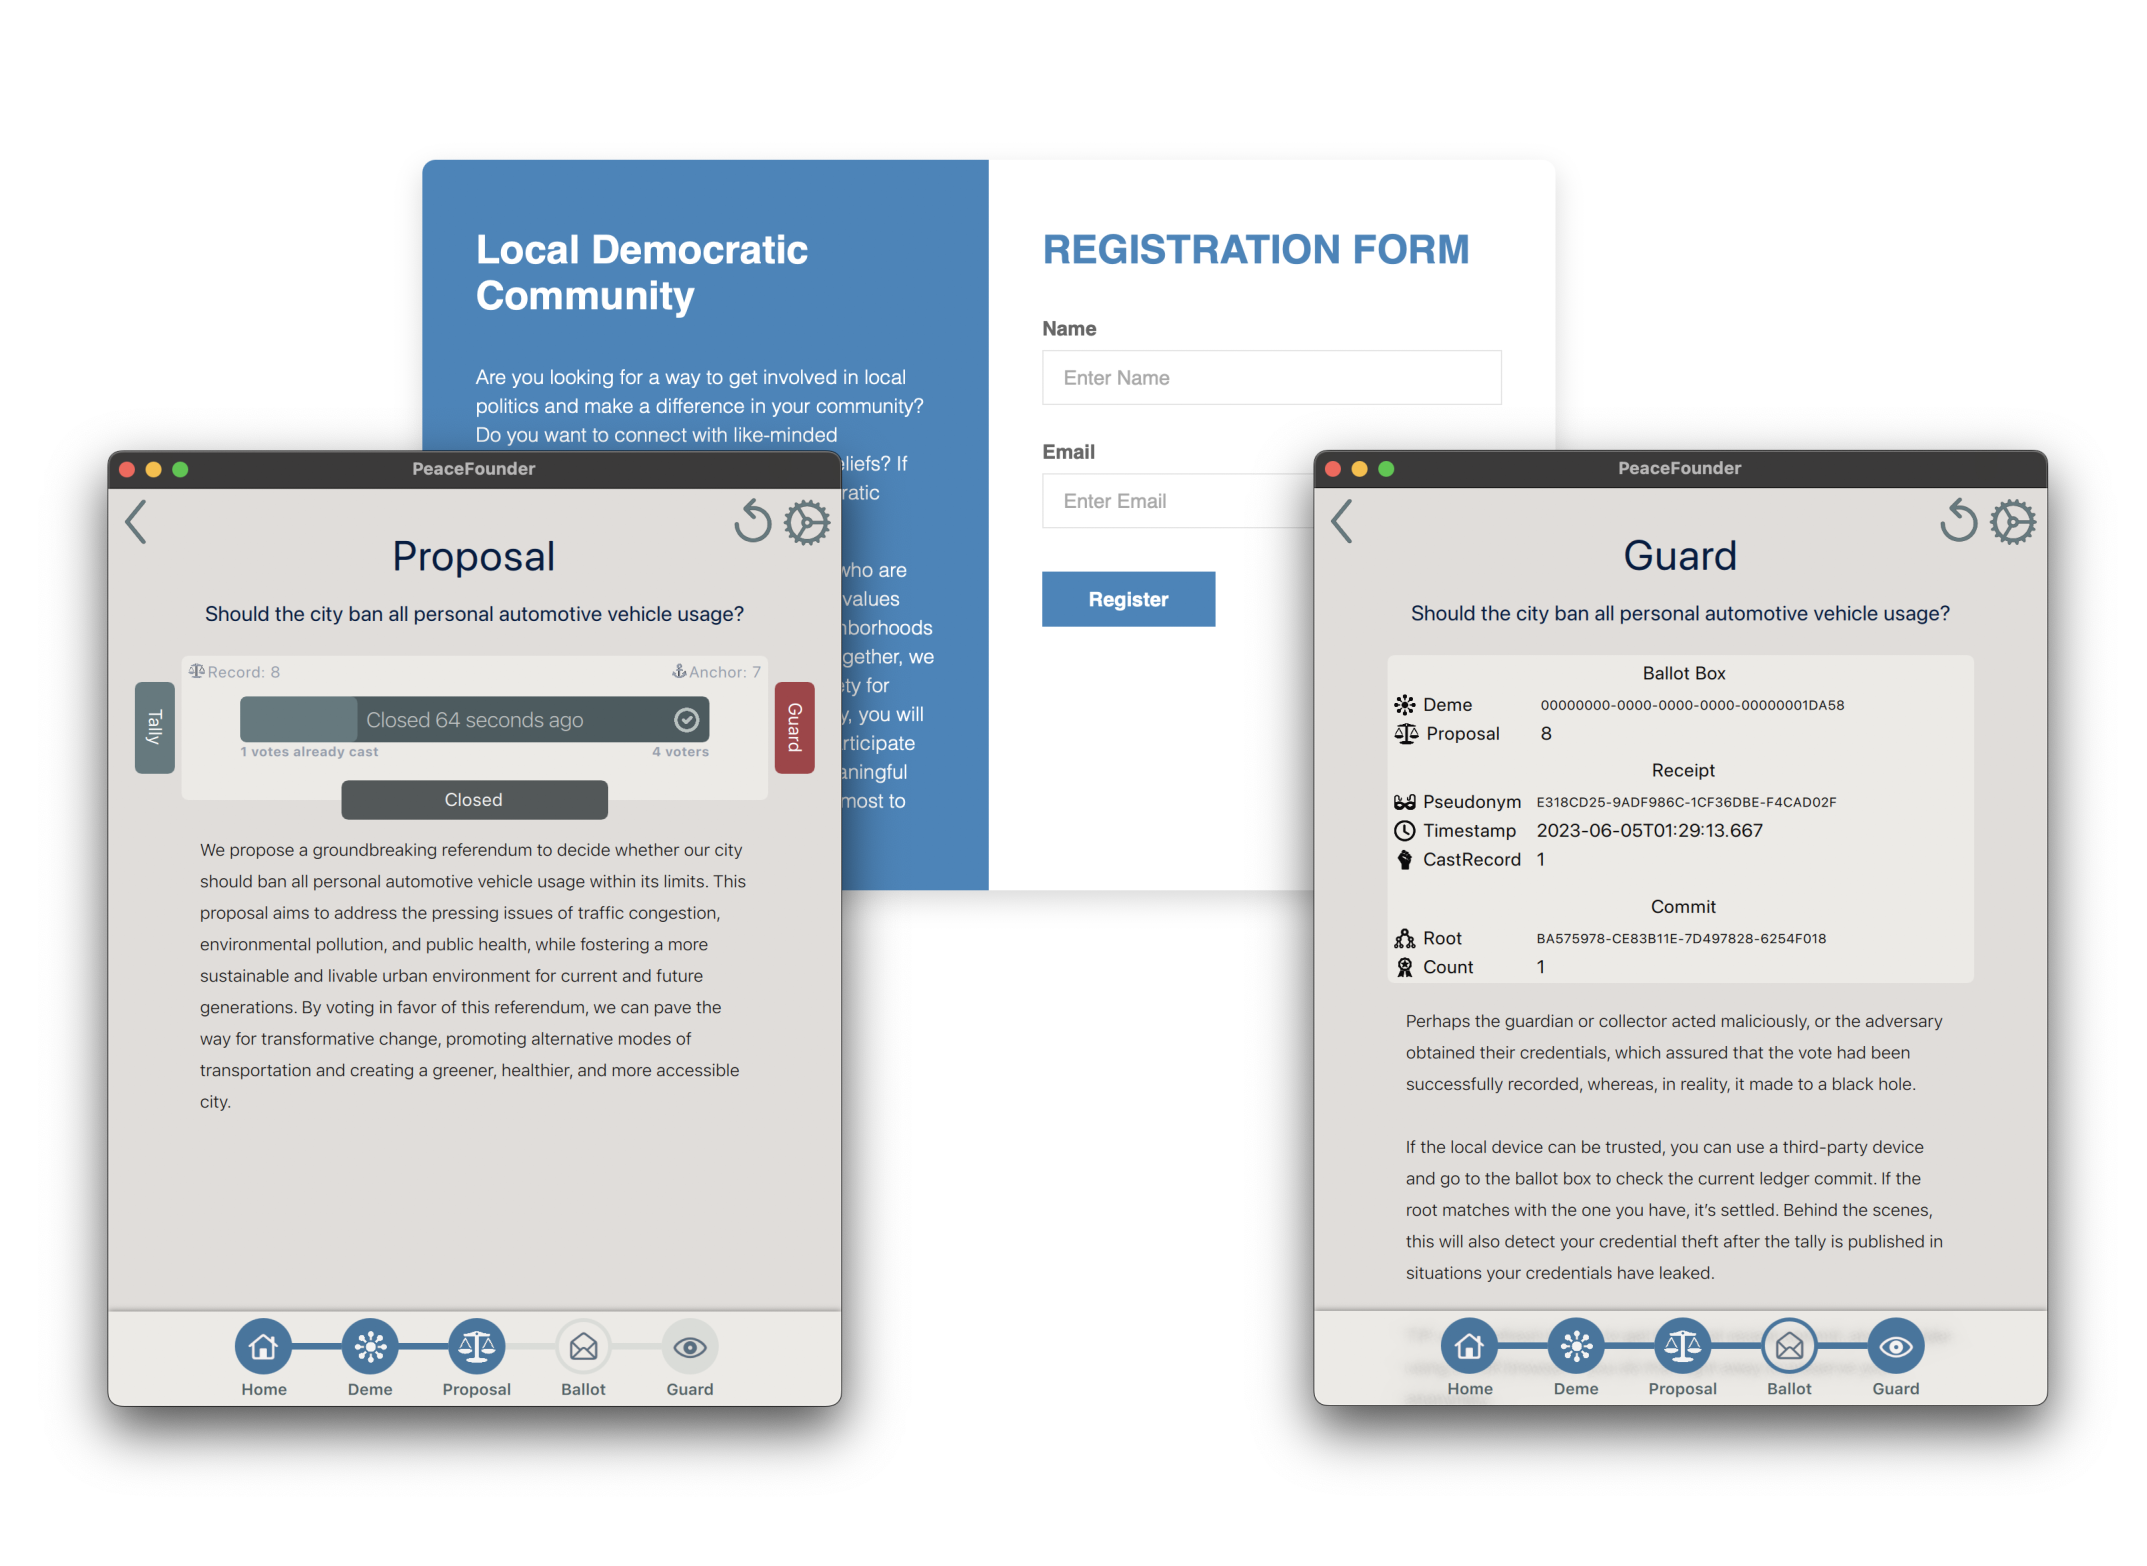
\includegraphics[width=\colwidth, trim=4.5cm 0cm 5cm 0cm]{figures/showcase.png}

  \begin{block}{Ballot Diversity \& Inovation}

    \begin{itemize}
    \item \textbf{Diverse Ballots:} As votes are in a plaintext signed by a pseudonym, it is trivial to support a diverse set of ballot types, including cardinal, budget planning and preferential ballots. It can also support internal whistleblowing.
    \item \textbf{Fluid Voting:} Pseudonymity enables fluid voting, letting voters revise their decisions within set periods during a representative term, bridging the gap between representative and direct democracy.
    \item \textbf{Ballot Sharding:} Long ballots can be divided into smaller shards and distributed among members' pseudonyms in a lottery. This elevates the impact of individual voters' choices, reduces the decision fatigue of a large ballot, and thus addresses the voting paradox.
    \end{itemize}
  \end{block}

  \begin{block}{Centralised Responsability}

    \begin{itemize}
    \item Built without a trusted quorum assumption, avoids threshold decryption ceremony and any trusted setup phase. 
    \item Braiding operates on a transactional basis, making it suitable for a market. Once a braid is computed, returned and verified, there’s no lingering trust assumption, allowing untrusted third parties from anywhere in the world to engage in anonymization.
    \item Leverages the power of voter devices to guarantee bulletin board record immutability with history tree consistency proofs. This oversight grows with member count and eliminates the need for bulletin board replication, offering both efficiency and reliability.
    \item Any misconduct results in publishable cryptographic evidence identifying responsible party, whether it’s the registrar, proposer, bulletin board, or braider authorities.
    \item The system can be easily set up and managed by just one person, or can be delegated for its deployment and maintenance to a third party.
    \end{itemize}
    
  \end{block}
  
  \begin{block}{E2E Verifiable with Coercion/Bribery Resistance}

    \begin{center}
      \vspace{-0.75cm}
      \includegraphics[width=\colwidth]{figures/e2e-properties.png}
      \vspace{-2.5cm}
    \end{center}

    \begin{itemize}
    \item Resistance to coercion and bribery hinges on the assumption that voters would not commit to distant positive/negative outcomes allowing them to freely revote or tag vote as coerced. We shall call this a moratorium period, within which there is a receipt-freeness but no public verifiability.
    \end{itemize}
    
    \begin{center}
      \vspace{-0.5cm}
      \includegraphics[width=0.5\colwidth]{figures/receipt-freeness.pdf}
      \vspace{-1cm}
    \end{center}
    
    \begin{itemize}
    \item The system is designed to resist malware and spyware. Voters can check if their vote was discarded or altered by comparing their receipt with the bulletin board’s records. Additionally, the device alerts the voter if a vote is cast outside the device, which can be cross-verified with the bulletin board. Note that the aim is to enable voters to detect malware interference; it’s not intended as a proof to be shown to a third party.
    \end{itemize}
    
  \end{block}

  
\end{column}

\separatorcolumn

\begin{column}{\colwidth}

\vspace{-5cm}
  
  \begin{block}{Responsabilities \& Interactions}

    \begin{itemize}
    \item Modular design and a public bulletin board allow seamless integration, facilitating custom dashboards on organisational websites.
    \item Custom registrars enable diverse identity authentication methods and third-party audit provisions. 
    \item Custom proposers can adapt to varied organisational proposal submission procedures. 
    \end{itemize}

    \begin{center}
      \includegraphics[width=0.65\colwidth]{figures/model-dependencies.pdf}
      \vspace{-1cm}
    \end{center}
    \begin{itemize}
    \item Auditors uphold the integrity of both BraidChain and BallotBox ledgers, ensuring accurate vote tallying and verifying voter eligibility. Additionally, they enhance bulletin board availability by relaying votes and document suspicious activities, and can relay unrecordable votes or blame proofs between themselves to reach a consensus, paving the way for judicial actions.
    \item Untrusted third parties can host braiders, ensuring unlinkability for voters. Self-braiding can be useful for sanitising public evidence. Deme-based braiding exchange ensures vote privacy against dishonest organisers. 
    \item To ensure voters' untraceability, votes are routed via the TOR service. Public IPs or domain names are recorded on the bulletin board to prevent segregation-type attacks. 
    \end{itemize}

    \begin{center}
      \includegraphics[width=\colwidth]{figures/model-responsabilities.pdf}  
      \vspace{-2cm}
    \end{center}
    
  \end{block}

  \begin{block}{Extensions}

    \begin{itemize}
    \item \textbf{Proof of Participation:} A bulletin board issues blind signatures on voters’ blinded identifiers included in the vote and are returned along with a receipt (assymetrically encrypted for unlinkability with a distinct key for each receipt), which voters devices unblind and can show to authority as proof of participation. After the moratorium, the signature is published on the bulletin board along with votes to avoid discrimination.
      
      \vspace{0.5em}
      
  To ensure authenticity, each pseudonym receives only one unique signature. The client device maintains a consistent, secretly and randomly generated blinding factor for all votes. As an added benefit, a bulletin board can detect private key leaks, and an invalid returned signature alerts the voter to a private key breach, promoting accountability by discouraging the use of leak-prone devices or practices.

\item \textbf{Selection Asymmetric Encryption:} To maintain the imparity of auditors/proxies with respect to the votes they receive and prevent coercers/bribers from seeing what vote they receive until the moratorium ends, the ballot selections for votes can be asymmetrically encrypted. Then, a proof of correct decryption is published on the bulletin board to ensure integrity. This also enables coerced vote tagging with a decoy PIN code when a coercer/briber is observing a voter in person. 

\item \textbf{Ballot Sharding:} The shards of the ballot are specified, and a lottery for them is set after the proposal is published on the bulletin board. When a verifiably random salt is generated with a service like DRAND, the member pseudonyms are hashed with this salt and sorted to which the shards are allocated in order. This prevents a small minority from conspiring and allocating important questions to themselves. 
    \end{itemize}

  \end{block}
  

  \begin{block}{References}

    \nocite{*}
    \footnotesize{\bibliographystyle{unsrt}\bibliography{poster}}

  \end{block}

\end{column}

\separatorcolumn
\end{columns}
\end{frame}

\end{document}

%%% Local Variables:
%%% mode: latex
%%% TeX-master: t
%%% End:
